% Chapter 3

\chapter{Solution n° 2} % Main chapter title

\label{Chapter3} % For referencing the chapter elsewhere, use \ref{Chapter3}
%----------------------------------------------------------------------------------------
\begin{description}
  \item[Version du Kernel :] 4.14
\end{description}

\section{Kernel 4.14}
La version 4.14 du kernel contient un driver imx219
main-line opérationel. Notre idée était de porter la meta-voipac compatible
avec un kernel 4.1 sur un kernel 4.14 pour pouvoir utiliser le driver.

\section{Travail effectué}
\textbf{Modifier les sources du Kernel}

 Dans les recettes chaque version du kernel est architecturée de la même façon :
  \begin{itemize}
  \item[-] un fichier linux-voipac\_4.14.bb
  \item[-] un dossier linux-voipac-4.14 contenant un defconfig et un patch du device tree de l'Openrex
  \end{itemize}

\begin{figure}[th]
  \centering
  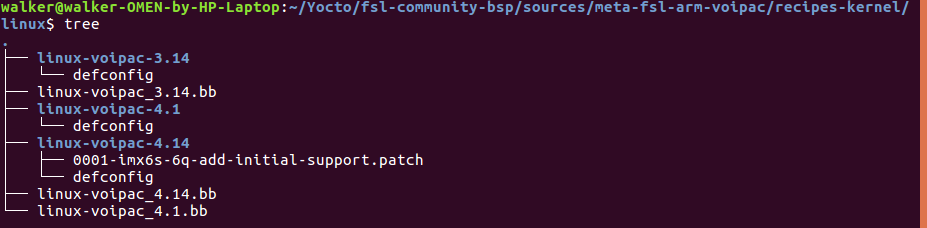
\includegraphics[width=1\linewidth]{tre.png}
  \decoRule
  \caption{Arborescence des fichiers}  \label{fig:arborescence4.14}
\end{figure}

Le principe de cette méthode est de copier la version 4.1 et de remplacer les sources du kernel. 

\begin{description}
  \item[Modification du fichier]
    \begin{lstlisting}
      SRCBRANCH = "4.14.x+fslc"
      LOCALVERSION = "-yocto"
      SRCREV = "${AUTOREV}"
      KERNEL_SRC ?= "git://github.com/Freescale/linux-fslc.git;protocol=git"
    \end{lstlisting}
\end{description}

\section{Erreur}
Nous obtenons quelques erreurs relative à gstreamer et alsa pendant la compilation du nouveau kernel.
Ces paquets n'étant pas essentiels à l'utilisation du driver nous les avons simplement enlevé les paquets.

L'étape de compilation réussite, nous obtenons une erreur lors du boot :
\begin{figure}[th]
  \centering
  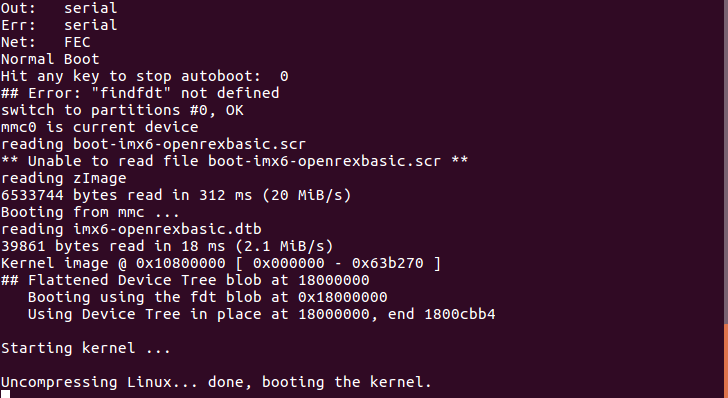
\includegraphics[width=1\linewidth]{4-14boot.png}
  \decoRule
  \caption{Erreur du bootloader}  \label{fig:planning}
\end{figure}

\section{Conclusion}

U-boot n'arrive pas à lancer notre image, il y a donc une imcompatibilitée entre 
la version du kernel et celle du bootloader chargée dans la SPI flash. Pour parvenir
à utiliser cette nouvelle image nous devons concevoir un nouveau bootlaoder en suivant
la méthode présentée
\href{http://www.imx6rex.com/open-rex/software/yocto-uboot-how-to-add-support-for-a-custom-board/}
{ici}.
 
\section{Reste à faire}
\begin{itemize}
\item[-] Créer un nouveau bootlaoder.
\item[-] Tester le nouveau bootlaoder.
\end{itemize}

%----------------------------------------------------------------------------------------
